\documentclass[preview]{standalone}
\usepackage{pgfplots}
\usepackage{amsmath}

\begin{document}
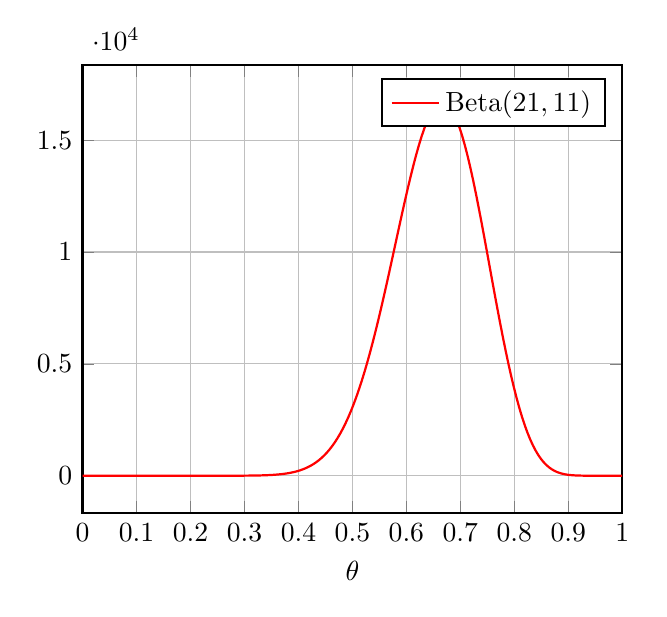
\begin{tikzpicture}
    \begin{axis}[
        domain=0:1,
        samples=200,
        thick,
        legend pos=north east,
        xlabel={$\theta$},
        grid=major,
        xmin=0, xmax=1,
        xtick={0,0.1,...,1},
    ]
        % Beta(21,11) -> B(21,11) ≈ 3.05e-13
        \addplot[red] {3.28e+12 * x^(21-1) * (1-x)^(11-1)};
        \addlegendentry{$\text{Beta}(21,11)$}
    \end{axis}
\end{tikzpicture}
\end{document}
